\part{\LaTeX}

Make guide on gloassaries and command:  \texttt{/setcounter (section) (-1)} - curly brackets and backslash\\
\Gls{paradigm}\\
\gls{paradigm}\\
\Glspl{paradigm}\\
\glspl{paradigm}\\
\acrshort{cpu}\\
\acrlong{cpu}\\
\acrfull{cpu}\\
\url{https://www.youtube.com/watch?v=PatWof0U-T8}

\section{Glossaries}

Subject of this topic is a brief tour around \textbf{glossaries}, which are defined as ``\textit{an alphabetical list of words relating to a specific subject, text, or dialect, with explanations; a brief dictionary}". To generate a glossary in an automatic manner \LaTeX\ uses a package called: \textbf{glossaries}. Like in most cases, we do want to specify additional parameters to the package, e.g. \textit{acronym}, \textit{toc}, \textit{section=section}.\\

Before processing any code one thing has to be mentioned. This package requires custom compilation scheme. Unfortunately there is no preset built into \textbf{TeXMaker} for a compilation scheme that will proces glossaries. A command chain has to be configured manually.

\begin{figure}[H]
\centering
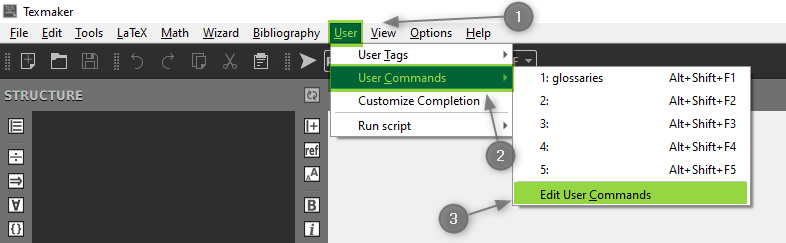
\includegraphics[scale=0.6]{LaTeX/figures/user_command_glossaries_marked.png}
\caption{Location of \textbf{Edit User Commands} button in \textbf{TeXMaker} environment}
\end{figure}

In order to do that, go to: \textbf{User} -> \textbf{User Commands} -> \textbf{Edit User Commands} and type below code into \textbf{command} field:
\begin{verbatim}
pdflatex -synctex=1 -interaction=nonstopmode %.tex | makeglossaries % | pdflatex 
-synctex=1 -interaction=nonstopmode %.tex | "C:/Program Files (x86)/Adobe/Acrobat
Reader DC/Reader/AcroRd32.exe" %.pdf
\end{verbatim}

\begin{figure}[H]
\centering
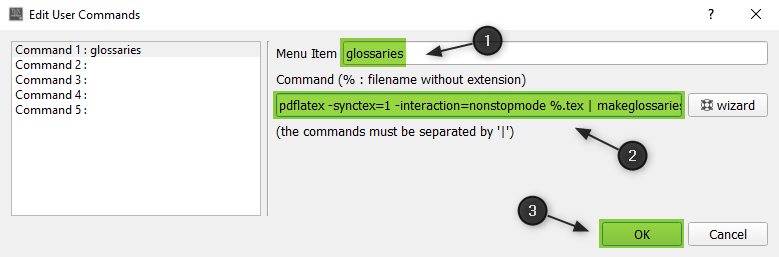
\includegraphics[scale=0.6]{LaTeX/figures/custom_command_marked.png}
\caption{Layout of \textbf{Edit User Commands} window in \textbf{TeXMaker} environment}
\end{figure}

Pipe symbol is used to chain commands. Words preceded by pause: ``-" are parameters passed to commands, which are words without any additions, placed at the beginning of every part - right after pipe or at the very beginning. Disassembly of this chain of commands allows to differentiate four differents parts here:
\begin{enumerate}
\item Generate \textbf{.pdf} file from the \textbf{.tex} file
\item Generate glossaries
\item Generate \textbf{.pdf} file from the \textbf{.tex} file
\item Display \textbf{.pdf}
\end{enumerate}
\fbox{\textcolor{red}{use figures in figures->TO USE}}\\
\fbox{\textcolor{red}{types of glossary entries}}\\
\fbox{\textcolor{red}{commands used to define glossary entries}}\\
\fbox{\textcolor{red}{commands used to refer to the glossary entries}}\\
\fbox{\textcolor{red}{commands used to generate glossary at the end - it is generated only when references are used in the text}}\\
\fbox{\textcolor{red}{commands used to customize display of the glossary}}

\begin{verbatim}

%\glossarystyle{listhypergroup} ????

% acronym - allows create different table for acronyms
% toc,section=section - allows glossaries to be printed in table of contents

\makeglossaries

\newglossaryentry{paradigm}
{
    name=paradigm,
    description={a typical example or pattern of something; a pattern or model}
}

\newacronym{cpu}{CPU}{Central Processing Unit}

%\glossarystyle{listhypergroup}
\printglossary[title=Skróty, toctitle=Skróty z kosmosu,type=\acronymtype]



\printglossary[title=Kosmiczny glosariusz, toctitle=Kosmiczne pojęcia] 
\end{verbatim}

\section{Quotes}

There are several types of quoting avaliable in \LaTeX.

Symbol that is placed on the same key as \textbf{tilde} (under or next to the \textbf{escape} button), is used to generate right facing quotes used in anglo-saxon quoting notation.

\fbox{\textcolor{red}{To finish}}

\section{Writing your own class}

\fbox{\textcolor{red}{To be implemented}}

\section{Writing your own package}

\fbox{\textcolor{red}{To be implemented}}

\section{Description list environment}

Next to \textbf{Itemize} and \textbf{Enumerate} there is \textbf{Description} list environment in \LaTeX . It's a glossary type of list environment consisting of key-value data records. e.g.

\begin{description}
\item[Item one] description of item one
\item[item two] description of item two
\item[item three] description of item three
\end{description} 

Above structure is generated by code:

\begin{verbatim}
\begin{description}
\item[Item one] description of item one
\item[item two] description of item two
\item[item three] description of item three
\end{description} 
\end{verbatim}


